
\setcounter{ex}{0}\setcounter{ex}{0}
\Opensolutionfile{ans}[ans/ans-KT-301]

\begin{ex} 
	Giá trị lượng giác nào sau đây là số dương?
	\choice
	{\True $\sin 120^\circ$}
	{$\cos 137^\circ$}
	{$\tan 160^\circ$}
	{$\cot 160^\circ$}
	\loigiai{
		Ta có $90^\circ<120^\circ<180^\circ$ nên $\sin 120^\circ>0$.\\
		Do $90^\circ<137^\circ<180^\circ$ nên $\cos 137^\circ<0$.\\
		Ngoài ra, $90^\circ<160^\circ<180^\circ$ nên $\tan 160^\circ<0$ và $\cot 160^\circ<0$.
	}
\end{ex}

\begin{ex}
	Cho $\sin\alpha=\dfrac{4}{5}$, $\left(90^\circ<\alpha <180^\circ\right)$. Tính $\cos\alpha $.
	\choice
	{$\cos\alpha=-\dfrac{4}{5}$}
	{\True $\cos\alpha=-\dfrac{3}{5}$}
	{$\cos\alpha=\dfrac{5}{3}$}
	{$\cos\alpha=\dfrac{3}{5}$}
	\loigiai{
		Ta có $\sin^2\alpha+\cos^2\alpha=1$ $\Leftrightarrow \cos^2\alpha=1-\sin^2\alpha=1-\dfrac{16}{25}=\dfrac{9}{25}\Rightarrow\cos\alpha=\pm\dfrac{3}{5}$.\\
		Mặt khác $90^\circ<\alpha<180^\circ$ nên $\cos\alpha=-\dfrac{3}{5}$.}
\end{ex}

\begin{ex}
	Cho $x\in\left(0^\circ;90^\circ\right)$. Phát biểu nào sau đây là đúng?
	\choice
	{\True $\sin x>0$}
	{$\cos x>0$}
	{$\tan x>0$}
	{$\cot x>0$}
	\loigiai{
		Khi $x\in\left(\dfrac{5\pi}{2};3\pi\right)$ thì $\heva{&\sin x>0\\&\cos x<0\\&\tan x<0\\&\cot x<0.}$ }  
\end{ex}
\begin{ex}
	Giá trị $\cos 45^\circ+\sin 45^\circ$ bằng bao nhiêu?
	\choice
	{$1$}
	{\True $\sqrt{2}$}
	{$\sqrt{3}$}
	{$0$}
	\loigiai
	{Bằng cách tra bảng giá trị lượng giác của các góc đặc biệt hay dùng MTCT ta được $\heva{& \cos 45^\circ=\dfrac{\sqrt{2}}{2} \\ 
			& \sin 45^\circ=\dfrac{\sqrt{2}}{2} \\ 
		}$\\
		$\Rightarrow \cos 45^\circ+\sin 45^\circ=\sqrt{2}$.}
\end{ex}
\begin{ex}
	Giá trị của $\cot18^\circ$ là
	\choice
	{$1$}
	{$-1$}
	{$0$}
	{\True $\sqrt{5+2\sqrt{5}}$}
	\loigiai{
		Ta có $\cot18^\circ=\sqrt{5+2\sqrt{5}}$.
	}
\end{ex}
\begin{ex}
	Trên nửa đường tròn đơn vị cho góc $\alpha$ sao cho $\sin\alpha=\dfrac{2}{3}$ và $\cos\alpha<0$. Tính $\tan\alpha$.
	\choice
	{\True $-\dfrac{2\sqrt{5}}{5}$}
	{$\dfrac{2\sqrt{5}}{5}$}
	{$-\dfrac{2}{5}$}
	{$1$}
	\loigiai{
		Ta có $\cos\alpha=-\sqrt{1-\sin^2\alpha}=-\dfrac{\sqrt{5}}{3}$ suy ra $\tan\alpha=-\dfrac{2\sqrt{5}}{5}$.
	}
\end{ex}
\begin{ex}
	Cho $\sin x+\cos x=\dfrac{1}{2}$ và $0<x<90^\circ$. Tính giá trị của $\sin x$
	\choice
	{$\sin x=\dfrac{1+\sqrt{7}}{-6}$}
	{$\sin x=\dfrac{1-\sqrt{7}}{6}$}
	{\True $\sin x=\dfrac{1+\sqrt{7}}{4}$}
	{$\sin x=\dfrac{1-\sqrt{7}}{4}$}
	\loigiai{
		Vì $0<x<90^\circ$ nên $\sin x>0$. Ta có
		\begin{eqnarray*}
			\sin^2x+\cos^2x=1 &\Leftrightarrow&\sin^2x+\left( \dfrac{1}{2}-\sin x\right)^2 =1\\
			&\Leftrightarrow& 2\sin^2x-\sin x-\dfrac{3}{4}=0\\
			&\Leftrightarrow& \hoac{&\sin x=\dfrac{1+\sqrt{7}}{4}\\&\sin x=\dfrac{1-\sqrt{7}}{4} \text{ (loại).}}
		\end{eqnarray*}
	}
\end{ex}  
\begin{ex} 
	Chọn phát biểu đúng trong các phát biểu sau?
	\choice
	{$\sin 156^\circ\cdot\cos70^\circ<0$}
	{$\tan 137^\circ\cdot\tan 156^\circ<0$}
	{\True $\tan150^\circ\cdot\cot85^\circ<0$}
	{$\sin 110^\circ\cdot\cos 110^\circ>0$}
	\loigiai{
		\begin{enumerate}
			\item Do $\heva{&\sin156^\circ>0\\&\cos70^\circ>0}$ nên $\sin 156^\circ\cdot \cos(-70^\circ)>0$.
			\item Do $\heva{&\tan 137^\circ<0\\&\tan 156^{\circ}<0}$ nên $\tan 137^\circ\cdot \tan 156^\circ>0$.
			\item Do $\heva{&\tan 150^\circ>0\\&\cot 85^\circ>0}$ nên $\tan 150^\circ\cdot\cot 85^\circ<0$.
			\item Do $\heva{&\sin 110^\circ>0\\&\cos 110^\circ<0}$ nên $\sin 110^\circ\cdot\cos 110^\circ<0$.
		\end{enumerate}
	}
\end{ex}
\begin{ex} 
	Phát biểu nào sau đây là đúng?
	\choice
	{$\sqrt{1-\sin^2 140^\circ}=\cos 140^\circ$}
	{\True $\sqrt{1-\cos^2 140^\circ}=\sin 140^\circ$}
	{$\sqrt{\dfrac{1}{\cos^2 140^\circ}-1}=\tan 140^\circ$}
	{$\dfrac{1}{\sqrt{\tan^2 140^\circ+1}}=\cos 140^\circ$}
	\loigiai{
		Do $140^\circ\in\left(90^\circ;180^\circ\right)$ nên $\heva{&\sin 140^\circ>0\\&\cos 140^\circ<0\\&\tan 140^\circ<0\\&\cot 140^\circ<0}$ nên $\heva{&\sqrt{1-\sin^2 140^\circ}=-\cos 140^\circ\\ &\sqrt{1-\cos^2 140^\circ}=\sin 140^\circ\\& \sqrt{\dfrac{1}{\cos^2 140^\circ}-1}=-\tan 140^\circ\\ &\dfrac{1}{\sqrt{\tan^2 140^\circ+1}}=-\cos 140^\circ.}$
	}   
\end{ex}
\begin{ex}
	Tìm mệnh đề \textbf{sai} trong các mệnh đề sau
	\choice
	{$\cos 0^\circ=1$}
	{$\sin 0^\circ=0$}
	{\True $\cos 120^\circ=\dfrac{2}{\sqrt{2}}$}
	{$\sin 120^\circ=\dfrac{\sqrt{3}}{2}$}
	\loigiai{
		Mệnh đề sai là $\cos 120^\circ=\dfrac{2}{\sqrt{2}}$ vì $\cos 120^\circ=-\cos 60^\circ=\dfrac{\sqrt{3}}{2}$.
}
\end{ex}
\begin{ex}
	Cho $\alpha$ là góc tù. Mệnh đề nào đúng trong các mệnh đề sau?
	\choice
	{$\sin\alpha<0$}
	{$\cos\alpha>0$}
	{\True $\tan\alpha<0$}
	{$\cot\alpha>0$}
	\loigiai{
		Vì $\alpha$ là góc tù nên $\tan\alpha<0$.
}
\end{ex}
\begin{ex}
	Trong các mệnh đề sau, mệnh đề nào \textbf{sai}?
	\choice
	{$\cos 45^\circ=\sin 45^\circ$}
	{$\cos 45^\circ=\sin 135^\circ$}
	{$\cos 30^\circ=\sin 120^\circ$}
	{\True $\sin 60^\circ=\cos 120^\circ$}
	\loigiai{
		Ta có $\sin 60^\circ=\dfrac{\sqrt{3}}{2}$ và $\cos 120^\circ=-\cos 60^\circ=-\dfrac{1}{2}$.\\
		Do đó mệnh đề sai là $\sin 60^\circ=\cos 120^\circ$.
}
\end{ex}
\begin{ex}
	Cho hai góc nhọn $\alpha$ và $\beta$ với $\alpha<\beta$. Tìm mệnh đề \textbf{sai}.
	\choice
	{$\sin\alpha<\sin\beta$}
	{\True $\cos\alpha<\cos\beta$}
	{$\cos\alpha=\sin\beta\Leftrightarrow \alpha+\beta=90^\circ$}
	{$\tan\alpha+\tan\beta>0$}
	\loigiai{
		Ta có mệnh đề \textbf{sai} là $\cos\alpha<\cos\beta$.
}
\end{ex}
\begin{ex}
	Cho $0^{\circ}\leq\alpha\leq 180^{\circ}$. Khẳng định nào sau đây là đúng?
	\choice
	{\True $\sin\alpha=\sin(180^{\circ}-\alpha)$}
	{$\cos\alpha=\cos(180^{\circ}-\alpha)$}
	{$\tan\alpha=\tan(180^{\circ}-\alpha)$}
	{$\cot\alpha=\cot(180^{\circ}-\alpha)$}
	\loigiai{
		Khẳng định đúng là $\sin\alpha=\sin(180^{\circ}-\alpha)$.
}
\end{ex}
\begin{ex}
	\immini{Trên nửa đường tròn đơn vị, vị trí nào trong các vị trí dưới đây xác định điểm $M$ sao cho $\tan\widehat{xOM}=1$.
		\choice
		{\True Vị trí $(1)$}
		{Vị trí $(2)$}
		{Vị trí $(3)$}
		{Vị trí $(4)$}
	}
	{
		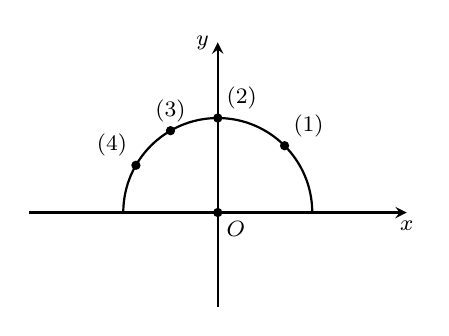
\begin{tikzpicture}[>=stealth,x=1.0cm,y=1.0cm,thick,scale=1.2]
		\begin{footnotesize}
		\draw[->] (-2,0) -- (2,0) node[below] {$x$};
		\draw[->] (0,-1) -- (0,1.8) node[left] {$y$};
		\coordinate (O) at (0,0);
		\fill[black] (0,0) circle[radius=1.4pt] node[below right]{\footnotesize $O$};
		\coordinate (M) at (0.7071,0.7071);
		\fill[black] (0.7071,0.7071) circle[radius=1.4pt] node[above right]{\footnotesize $(1)$};
		\draw (1,0) arc (0:180:1);
		\coordinate (P) at (-0.866,0.5);
		\fill[black] (-0.866,0.5) circle[radius=1.4pt] node[above left]{\footnotesize $(4)$};
		\coordinate (N) at (-0.5,0.866);
		\fill[black] (-0.5,0.866) circle[radius=1.4pt] node[above ]{\footnotesize $(3)$};
		\coordinate (Q) at (0,1);
		\fill[black] (0,1) circle[radius=1.4pt] node[above right]{\footnotesize $(2)$};
		
		\end{footnotesize}
		\end{tikzpicture}
	}	
	\loigiai{
		Ở vị trí $1$ ta có $\sin\widehat{xOM}=\cos\widehat{xOM}$ nên $\tan\widehat{xOM}=1$.
}
\end{ex}
\begin{ex}
	Cho hai góc $\alpha$ và $\beta$ với $\alpha+\beta =180^\circ$. Tính giá trị của biểu thức $P=\cos\alpha\cos\beta -\sin\beta\sin\alpha$.
	\choice
	{$P=0$}
	{$P=1$}
	{\True $P=-1$}
	{$P=2$}
	\loigiai
	{Hai góc $\alpha$ và $\beta$ bù nhau nên $\sin\alpha =\sin\beta$; $\cos\alpha =-\cos\beta$.\\
	Do đó $P=\cos\alpha\cos\beta -\sin\beta\sin\alpha =-\cos^2\alpha -\sin^2\alpha =-(\sin^2\alpha +\cos^2\alpha)=-1$.}
\end{ex}
\begin{ex}
	Khẳng định nào sau đây \textbf{sai}?
	\choice
	{\True $\cos 75^\circ >\cos 50^\circ $}
	{$\sin 80^\circ >\sin 50^\circ $}
	{$\tan 45^\circ <\tan 60^\circ $}
	{$\cos 30^\circ =\sin 60^\circ $}
	\loigiai
	{Trong khoảng từ $0^\circ$ đến $90^\circ$, khi giá trị của góc tăng thì giá trị $\cos$ tương ứng của góc đó giảm.}
\end{ex}
\begin{ex}
	Cho tam giác $MNP$ không vuông có diện tích là $S$, $p$ là nửa chu vi, $r$ là bán kính đường tròn nội tiếp và $R$ là bán kính đường tròn ngoại tiếp. Khẳng định nào sau đây là khẳng định \textbf{sai}?
	\choice
	{\True $S=\dfrac{1}{2}MN\cdot MP$}
	{$S=p\cdot r$}
	{$S=\dfrac{MN\cdot MP\cdot NP}{4R}$}
	{$S=\dfrac{1}{2}NM\cdot NP\cdot\sin{N}$}
	\loigiai{
		Khẳng định \textbf{sai} là $S=\dfrac{1}{2}MN\cdot MP$.
}
\end{ex}
\begin{ex}
	Tam giác $ABC$ vuông tại $A$ và có $AB=AC=a$. Tính độ dài đường trung tuyến $BM$ của tam giác đã cho.
	\choice
	{\True $BM=\dfrac{\sqrt{5}}{2}a$}
	{$BM=1{,}5a$}
	{$BM=\sqrt{2}a$}
	{$BM=\sqrt{3}a$}
	\loigiai{
		\immini{
			$M$ là trung điểm của $AC\Rightarrow AM=\dfrac{AC}{2}=\dfrac{a}{2}$.\\
			Xét tam giác $BAM$ vuông tại $A$, ta có\\
			$BM=\sqrt{AB^2+AM^2}=\sqrt{a^2+\dfrac{a^2}{4}}=\dfrac{a\sqrt{5}}{2}$.}
		{
			\begin{tikzpicture}[scale=1,font=\footnotesize,line join=round, line cap=round,>=stealth]
			\tkzDefPoints{0/0/A,0/3/B,4/0/C}
			\tkzDefMidPoint(A,C) \tkzGetPoint{M}
			\tkzDrawPoints[fill=black](A,B,C,M)
			\tkzDrawPolygon(A,B,C)
			\tkzDrawSegments(B,M)
			\tkzLabelPoints[above](B)
			\tkzLabelPoints[below](M,C,A)
			\tkzMarkRightAngles[size=0.2](C,A,B)
			\end{tikzpicture}
		}
	}
\end{ex}
\begin{ex}
	Cho tam giác $ABC$ có $3$ cạnh là $4$ cm, $8$ cm và $6$ cm. Tính bán kính $r$ của đường tròn nội tiếp tam giác $ABC$.
	\choice
	{$r=\dfrac{\sqrt{5}}{3}$ cm}
	{$r=\sqrt{5}$ cm}
	{$r=\sqrt{15}$ cm}
	{\True $r=\dfrac{\sqrt{15}}{3}$ cm}
	\loigiai{
		Ta có nửa chu vi $\triangle ABC$ là $p=\dfrac{4+8+6}{2}=9$ cm.\\
		Diện tích $\triangle ABC$ là $S_{\triangle ABC}=\sqrt{9(9-4)(9-6)(9-8)}=3\sqrt{15}$ cm $^2$.\\
		Suy ra bán kính $r$ của đường tròn nội tiếp tam giác $ABC$ là $r=\dfrac{S_{\triangle ABC}}{p}=\dfrac{3\sqrt{15}}{9}=\dfrac{\sqrt{15}}{3}$ cm.
}
\end{ex}
\begin{ex}
	Cho tam giác $ABC$ có $\widehat{A}=30^\circ$, $\widehat{B}=45^\circ$ và $AC=10\sqrt{2}$. Độ dài cạnh $BC$ là
	\choice
	{\True $10$}
	{$5\sqrt{2}$}
	{$\dfrac{5}{\sqrt{2}}$}
	{$5$}
	\loigiai{
		Ta có $\dfrac{AC}{\sin B}=\dfrac{BC}{\sin A}\Rightarrow BC=\dfrac{AC\cdot\sin A}{\sin B}=\dfrac{10\sqrt{2}\cdot\sin 30^\circ}{\sin 45^\circ}=10$.
}
\end{ex}
\begin{ex}
	Cho tam giác $ABC$. Khẳng định nào sau đây là đúng?
	\choice
	{$S=\dfrac{abc}{4r}$}
	{\True $r=\dfrac{2S}{a+b+c}$}
	{$a^2=b^2+c^2+2bc\cos A$}
	{$S=r(a+b+c)$}
	\loigiai{
		Gọi $a$, $b$, $c$ lần lượt là độ dài ba cạnh của tam giác $ABC$.\\
		Tam giác $ABC$ có nửa chi vi là $p=\dfrac{a+b+c}{2}$.\\
		Ta có $S=pr$. Suy ra $r=\dfrac{S}{p}=\dfrac{S}{\dfrac{a+b+c}{2}}=\dfrac{2S}{a+b+c}$.
	}
\end{ex}
\begin{ex}
	Tính diện tích của tam giác $ABC$ có $b=2$, $\widehat{B}=30^\circ$, $\widehat{C}=45^\circ$.
	\choice
	{$2+2\sqrt{3}$}
	{$1$}
	{$\sqrt{3}$}
	{\True $1+\sqrt{3}$}
	\loigiai{
		Ta có: $\dfrac{b}{\sin B}=\dfrac{c}{\sin C}$. \\
		Suy ra $c=\dfrac{b\cdot \sin C}{\sin B}=\dfrac{2\cdot \sin 45^\circ}{\sin 30^\circ}=2\sqrt{2}$.\\
		Ta có $\widehat{A}=180^\circ-\widehat{B}-\widehat{C}=180^\circ-30^\circ-45^\circ=105^\circ$.\\
		Ta có $S=\dfrac{1}{2}bc\sin A=\dfrac{1}{2}\cdot 2\cdot 2\sqrt{2}\cdot \sin 105^\circ=1+\sqrt{3}$.
	}
\end{ex}
\begin{ex}
	Trong tam giác $ABC$ có góc $\widehat{A}=60^{\circ}$, $AC=10$, $AB=6$. Khi đó, độ dài cạnh $BC$ là
	\choice
	{\True $2\sqrt{19}$}
	{$76$}
	{$14$}
	{$6\sqrt{2}$}
	\loigiai{
		Ta có: $BC^2=AB^2+AC^2-2AB\cdot AC\cos A=6^2+10^2-2\cdot 6\cdot 10\cdot\cos 60^{\circ}=76$.\\
		Suy ra $BC=2\sqrt{19}$.
	}
\end{ex}
\begin{ex}
	Cho $\triangle ABC$ có $AB=6$ cm, $BC=7$ cm, $CA=8$ cm. Giá trị của $\cos B$ là
	\choice
	{$\dfrac{1}{2}$}
	{\True $\dfrac{1}{4}$}
	{$\dfrac{17}{32}$}
	{$\dfrac{11}{16}$}
	\loigiai{
		Ta có $\cos B=\dfrac{AB^2+BC^2-AC^2}{2\cdot AB\cdot BC}=\dfrac{6^2+7^2-8^2}{2\cdot 6\cdot 7}=\dfrac{1}{4}$.
	}
\end{ex}
\begin{ex} 
	\immini{
		Để đo khoảng cách từ $A$ đến $B$ ngang qua một cái hồ nước, người ta chọn điểm  $C$, sau đó đo độ dài các cạnh $AC$, $BC$ và góc $C$.  Biết $AC=112$ m, $BC=145$ m, $\widehat{C}=75^\circ$, khoảng cách từ $A$ đến $B$ gần nhất với giá trị nào dưới đây?
		\choice
		{$155$ m}
		{\True $160$ m}
		{$165$ m}
		{$170$ m}
	}
	{
		\begin{tikzpicture}[scale=1, font=\footnotesize, line join=round, line cap=round,>=stealth]
		\path
		(2,2) coordinate (A)
		(7,2) coordinate (B)
		(2.5,2) coordinate (D)
		(3.5,3.1) coordinate (E)
		(5.5,2.9) coordinate (F)
		(6.4,1.5) coordinate (G)
		(5.2,0.7) coordinate (H)
		(3.5,0.7) coordinate (I)
		(2.6,1.3) coordinate (J)
		;
		\coordinate (C) at ($(A)+(53.6:3.6)$) ; 
		\draw[fill=cyan!40] 
		(D) 
		.. controls ++(65:0.1) and ++(200: 1) .. (E)
		.. controls ++(200:-0.5) and ++(170: 0.3) .. (F)
		.. controls ++(170:-0.5) and ++(100: 0.3) .. (G)
		.. controls ++(100:-0.3) and ++(30: 0.3) .. (H)
		.. controls ++(30:-0.3) and ++(150: -0.3) .. (I)
		.. controls ++(150:0.3) and ++(130: -0.3) .. (J)
		.. controls ++(130:0.3) and ++(65: -0.1) .. (D)
		;
		\draw[dashed] (D)--(6.2,2) ;
		\draw (A)--(C)--(B)  (A)--(D) (B)--(6.2,2) ;
		\draw pic["$75^{\circ}$", draw=black, angle eccentricity=1.4, angle radius=0.5cm]{angle=A--C--B};
		\foreach \x/\g in {A/-120,B/-60,C/90} 
		\fill[black] (\x) circle (1pt)+(\g:3mm) node {$\x$};
		\end{tikzpicture}
	}
	\loigiai{
		Áp dụng định lí côsin ta có 
	\begin{eqnarray*}
		&AB^2&=AC^2+BC^2-2AC\cdot BC\cos C\\
		&&=112^2+145^2-2\cdot 112\cdot 145\cos 75^\circ\\
		&&\Rightarrow AB\approx 158{,}6.
	\end{eqnarray*}	
	}
\end{ex}
\begin{ex}
	\immini{
		Để đo chiều cao $CH$ của một  tháp truyền thông, người ta chọn hai điểm quan sát $A$, $B$ trên mặt đất (hình vẽ). Biết $\widehat{CAH}=50^\circ$, $\widehat{CBH}=60^\circ$ và $AB=80$ m, tính chiều cao của tháp.
		\choice
		{$300{,}3$ m}
		{\True $305{,}6$ m}
		{$301{,}8$ m}
		{$306{,}9$ m}
	}
	{
		\begin{tikzpicture}[scale=1, font=\footnotesize, line join=round, line cap=round,>=stealth]
		\path
		(1,0) coordinate (A)
		(2,0) coordinate (B)
		(4,3.5) coordinate (C)
		(4,0) coordinate (H)
		;
		\draw [fill=gray!40]
		(3.7,0)
		.. controls ++(50:0.5) and ++(265: 1) .. (C) 
		.. controls ++(-85:1) and ++(130: 0.5) .. (4.3,0)--cycle;
		\draw (A)--(C)--(H)--(A) (B)--(C) ;
		\draw pic["$50^{\circ}$", draw=black, angle eccentricity=1.6, angle radius=0.5cm]{angle=H--A--C};
		\draw pic["$60^{\circ}$", draw=black, double, angle eccentricity=1.6, angle radius=0.5cm]{angle=H--B--C};
		\foreach \x/\g in {A/-90,B/-90,C/90,H/-90} 
		\fill[black] (\x) circle (1pt)+(\g:3mm) node {$\x$};
		\end{tikzpicture}
	}
	
	\loigiai{
		Ta có $\widehat{ACB}=\widehat{CBH}=60^\circ-50^\circ=10^\circ$. \\
		Áp dụng định lí sin ta có
		\[
		\dfrac{AB}{\sin\widehat{ACB}}=\dfrac{BC}{\sin\widehat{CAH}}\Rightarrow BC=\dfrac{AB\sin\widehat{CAH}}{\sin\widehat{ACB}}=\dfrac{80\sin 50^\circ}{\sin 10^\circ}.
		\]
		Suy ra $CH=BC\sin\widehat{CBH}=\dfrac{80\sin 50^\circ\sin 50^\circ}{\sin 10^\circ}\approx 305{,}6$ m.
	}
\end{ex}
\begin{ex}
	Cho tam giác $ABC$ có $\widehat{B}=135^\circ$. Khẳng định nào sau đây là đúng?
	\choice
	{$S=\dfrac{1}{2}ca$}
	{$S=-\dfrac{\sqrt{2}}{4}ac$}
	{$S=\dfrac{\sqrt{2}}{4}bc$}
	{\True $S=\dfrac{\sqrt{2}}{4}ca$}
	\loigiai{
		Gọi $a$, $b$, $c$ lần lượt là độ dài ba cạnh của tam giác $ABC$.\\
		Ta có $S=\dfrac{1}{2}ac\sin B=\dfrac{1}{2}ac\cdot\sin 135^\circ=\dfrac{1}{2}\cdot\dfrac{\sqrt{2}}{2}\cdot ac=\dfrac{\sqrt{2}}{4}ac$.
	}
\end{ex}
\begin{ex}
	Cho $\triangle ABC$ có $S=84$, $a=13$, $b=14$, $c=15$. Độ dài bán kính đường tròn ngoại tiếp $R$ của tam giác trên là
	\choice
	{\True $8{,}125$}
	{$130$}
	{$8{,}5$}
	{$8$}
	\loigiai{
		Ta có $S=\dfrac{abc}{4R}\Rightarrow R=\dfrac{abc}{4S}=\dfrac{13\cdot 14\cdot 15}{4\cdot 84}=8{,}125$.
	}
\end{ex}
\begin{ex}
	Cho $\triangle ABC$ với các cạnh $AB=c$, $AC=b$, $BC=a$. Gọi $R$, $r$, $S$ lần lượt là bán kính đường tròn ngoại tiếp, nội tiếp và diện tích của tam giác $ABC$ . Trong các phát biểu sau, phát biểu nào sai?
	\choice
	{$S=\dfrac{abc}{4R}$ }
	{\True $R=\dfrac{a}{\sin A}$ }
	{$S=\dfrac{1}{2}ab\sin C$ }
	{$a^2+b^2-c^2=2ac\cos C$}
	\loigiai
	{
		Theo định lý sin trong tam giác, ta có $\dfrac{a}{\sin A}=2R$.
	}
\end{ex}
\begin{ex}
	Cho tam giác $ABC$ thỏa mãn hệ thức $b+c=2a$. Trong các mệnh đề sau, mệnh đề nào đúng?
	\choice
	{$\cos B+\cos C=2\cos A$}
	{\True $\sin B+\sin C=2\sin A$}
	{$\sin B+\sin C=\dfrac{1}{2}\sin A$}
	{$\sin B+\cos C=2\sin A$}
	\loigiai{
		Ta có $\dfrac{a}{\sin A}=\dfrac{b}{\sin B}=\dfrac{c}{\sin C}=2R \Leftrightarrow \left\{\begin{aligned}
		&a=2R\sin A\\
		&b=2R\sin B\\
		&c=2R\sin C.
		\end{aligned}\right. $\\
		Mà $b+c=2a\Leftrightarrow 2R\sin B+2R\sin C=4R\sin A\Leftrightarrow\sin B+\sin C=2\sin A$.}
\end{ex}
\begin{ex}
	Tam giác có độ dài ba cạnh là $3$, $8$, $9$. Góc lớn nhất của tam giác có số đo bằng bao nhiêu?
	\choice
	{$93{,}5^\circ$}
	{$88{,}6^\circ$}
	{\True $99{,}6^\circ$}
	{$101{,}3^\circ$}
	\loigiai{
		Góc lớn nhất $\alpha$ của tam giác là góc đối diện với cạnh lớn nhất của tam giác. \\
		Áp dụng định lí côsin ta có
		\[
		\cos\alpha=\dfrac{3^2+8^2-9^2}{2\cdot 3\cdot 8}=-\dfrac{1}{6}\Rightarrow\alpha\approx 99{,}6^\circ.
		\]
	}
\end{ex}
\begin{ex}
	\immini{
		Từ một vị trí quan sát $A$, một người nhìn đỉnh $B$ và chân $C$ của nhà cao tầng với các góc tương ứng là $43^{\circ}$ và $16^{\circ}$ so với phương nằm ngang. Biết chiều cao của tòa nhà là $18$ m, tính khoảng cách từ $A$ đến $C$ (làm tròn kết quả đến hàng phần mười).
		\choice
		{$27$ m}
		{$28$ m}
		{\True $29$ m}
		{$31$ m}
	}
	{
		\begin{tikzpicture}[scale=0.8,>=stealth, font=\footnotesize, line join=round, line cap=round]
		\path 
		(0,0) coordinate (A)
		(4,3) coordinate (B)
		(4,-1) coordinate (C) 
		(4,0) coordinate (H) 
		;
		\draw[pattern=bricks,pattern color=brown] (B)--(6,3)--(6,-1)--(4,-1)--(B);
		\foreach \i in {2,3,4,5}
		\draw[fill=white] ({4+1/3},{-1+(2/3)*(\i-1)})--({4+1/3},{-1+(2/3)*(\i-1)+0.5})--({4+2/3},{-1+(2/3)*(\i-1)+0.5})--({4+2/3},{-1+(2/3)*(\i-1)})--cycle 
		({5+1/3},{-1+(2/3)*(\i-1)})--({5+1/3},{-1+(2/3)*(\i-1)+0.5})--({5+2/3},{-1+(2/3)*(\i-1)+0.5})--({5+2/3},{-1+(2/3)*(\i-1)})--cycle;
		\draw[dashed](A)--(B)  (A)--(C) (A)--(H); 
		\draw pic["$43^{\circ}$", draw=black, angle eccentricity=1.4, angle radius=0.9cm]{angle=H--A--B};
		\draw pic["$16^{\circ}$", draw=black,double, angle eccentricity=1.5, angle radius=1.2cm]{angle=C--A--H};
		\foreach \x/\g in {A/180,B/90,C/140,H/145} 
		\fill[black] (\x) circle (1pt)+(\g:3mm) node {$\x$};
		\clip (-0.5,{-1-0.25}) rectangle (6.6,-1) ;
		\draw[fill=gray!30] (-0.5,-1)--(6.6,-1)--(6.6,{-1-0.25})--(-0.5,{-1-0.25})--cycle;
		\foreach \i in {1,2,...,35}
		\draw ({-0.5+0.2*(\i)},-1)--($({-0.5+0.2*(\i)},-1)+(-120:0.3)$) ;
		\end{tikzpicture}
	}
	\loigiai{
		Ta có $AH=BH\cot\widehat{BAH}=CH\cot\widehat{CAH}$. \\
		Suy ra 
		\begin{align*}
		&(BC-CH)\cot\widehat{BAH}=CH\cot\widehat{CAH}\\
		\Leftrightarrow &CH=\dfrac{BC\cot\widehat{BAH}}{\cot\widehat{CAH} +\cot\widehat{BAH}} \\
		\Leftrightarrow &CH=\dfrac{18\cot 43^\circ}{\cot 16^\circ+\cot 43^\circ}.
		\end{align*}
		Khoảng cách từ $A$ đến $C$ là
		\[ AC=\dfrac{CH}{\sin 16^\circ}=\dfrac{18\cot 43^\circ}{(\cot 16^\circ+\cot 43^\circ)\sin 16^\circ}\approx 15{,}4\text{ m.}\]
	}
\end{ex}
\begin{ex}
	Cho tam giác $ABC$ có ba cạnh $a$, $b$, $c$ và $m_a$; $m_b$; $m_c$ là ba đường trung tuyến lần lượt xuất phát từ $A$, $B$, $C$. Tính tổng $S=m_a^2+m_b^2+m_c^2$.
	\choice
	{$S=\dfrac{3}{2}(a^2+b^2+c^2)$}
	{$S=\dfrac{4}{9}(a^2+b^2+c^2)$}
	{$S=\dfrac{9}{4}(a^2+b^2+c^2)$}
	{\True $S=\dfrac{3}{4}(a^2+b^2+c^2)$}
	\loigiai{
		\begin{eqnarray*}
			&m_a^2=&\dfrac{b^2+c^2}{2}-\dfrac{a^2}{4}. \\
			&m_b^2=&\dfrac{a^2+c^2}{2}-\dfrac{b^2}{4}. \\
			&m_c^2=&\dfrac{a^2+b^2}{2}-\dfrac{c^2}{4}.
		\end{eqnarray*}
		Vậy $S=m_a^2+m_b^2+m_c^2=a^2+b^2+c^2-\dfrac{a^2+b^2+c^2}{4}=\dfrac{3}{4}\cdot(a^2+b^2+c^2)$.}
\end{ex}
\begin{ex}
Cho tam giác $ABC$ có $a=49{,}4$; $b=26{,}4$; $\widehat{C}=47^{\circ}20'$. Cạnh $c$ gần bằng với số nào sau đây?
\choice
{$38$}
{\True $37$}
{$39$}
{$36$}
\loigiai{
	Ta có: $c=\sqrt{a^2+b^2-2ab\cos 47^{\circ}20'} \approx 37$.}
\end{ex}

% \noindent\textbf{II. PHẦN TỰ LUẬN}
% \begin{ex}
% 	Cho $\tan x=-4$. Tính giá trị biểu thức sau $A=\dfrac{\sin^2x-\sin 2x-4\cos^2x}{\sin 2x-2\cos^2x}$.
% 	\loigiai{
% 		Ta có $\tan x=-4\Rightarrow\cos x\neq 0$. Chia hai tử và mẫu biểu thức $A$ cho $\cos^2x$.\\
% 		Khi đó $A=\dfrac{\sin^2x-\sin 2x-4\cos^2x}{\sin 2x-2\cos^2x}=\dfrac{\tan^2x-2\tan x-4}{2\tan x-2}=\dfrac{(-4)^2-2 \cdot (-4)-4}{2 \cdot (-4)-2}=-2$}
% \end{ex}
\begin{ex}
	Chứng minh biểu thức sau độc lập với đối với $x$.
	\[P=\dfrac{\tan^2 x-\cos^2 x}{\sin^2 x}+\dfrac{\cot^2 x-\sin^2 x}{\cos^2 x}.\]
	\loigiai{
		Ta có   
		\begin{eqnarray*}
			P&=&\dfrac{\tan^2 x-\cos^2 x}{\sin^2 x}+\dfrac{\cot^2 x-\sin^2 x}{\cos^2 x}\\&=&\dfrac{\tan^2 x}{\sin^2 x}-\dfrac{\cos^2 x}{\sin^2 x}+\dfrac{\cot^2 x}{\cos^2 x}-\dfrac{\sin^2 x}{\cos^2 x}\\
			&=&\tan^2 x(1+\cot^2 x)+\cot^2 x(1+\tan^2 x)-\tan^2 x-\cot^2 x\\&=&\tan^2 x+1+\cot^2 x+1-\tan^2 x-\cot^2 x\\
			&=&2.
		\end{eqnarray*}
		Vậy $P$ không phụ thuộc vào $x$.
	}
\end{ex}
\begin{ex}
	Cho tam giác $ABC$, chứng minh rằng
	 $\cos\dfrac{A}{2}=\sqrt{\dfrac{p(p-a)}{b c}}$.
	\loigiai{
		\begin{center}
			\begin{tikzpicture}[scale=1, font=\footnotesize, line join=round, line cap=round, >=stealth]
			\pgfmathsetmacro\a{4/sqrt(3)}
			\path (0,0)  coordinate(D) (\a,0)  coordinate(A) (5,0)  coordinate(C) (30:4) coordinate(B) ($(D)!0.5!(B)$) coordinate (I);
			\draw (D)--(B)--(C)--cycle (B)--(A)--(I);
			\foreach \x/\g in {A/-90,B/90,C/-90,D/-90,I/90}\draw[fill=black] (\x) circle (.03) + (\g:.3) node{$\x$};
			\end{tikzpicture}
		\end{center}
		Trên tia đối của tia $AC$ lấy $D$ thỏa $AD=AB=c$ suy ra tam giác $BDA$ cân tại $A$ và $\widehat{BDA}=\dfrac{1}{2} \widehat{BAC}$ (góc ngoài tam giác).
			Áp dụng định lý hàm số cô-sin cho $\triangle ABD$ ta có
			\allowdisplaybreaks
			\begin{eqnarray*}
				BD^{2}&=&AB^{2}+AD^{2}-2AB \cdot AD\cdot\cos\widehat{BAD} \\
				&=&2c^{2}-2c^{2}\cdot\cos\left(180^{\circ}-A\right)\\
				&=&2c^{2}(1+\cos A)=2c^{2}\left(1+\dfrac{b^{2}+c^{2}-a^{2}}{2bc}\right) \\
				&=&\dfrac{c}{b}(a+b+c)(b+c-a)=4c^2\cdot\dfrac{p(p-a)}{bc} \\
				\text {suy ra}\,\,  BD&=&2c\sqrt{\dfrac{p(p-a)}{bc}}.
			\end{eqnarray*}
			Gọi $I$ là trung điểm của $BD$ suy ra $AI \perp BD$.
			Trong tam giác $ADI$ vuông tại $I$, ta có
			$$
			\cos\dfrac{A}{2}=\cos \widehat{ADI}=\dfrac{DI}{AD}=\dfrac{BD}{2c}=\sqrt{\dfrac{p(p-a)}{bc}}.
			$$
			Vậy $\cos \dfrac{A}{2}=\sqrt{\dfrac{p(p-a)}{b c}}$.
		}
\end{ex}
\begin{ex}
	Cho tam giác $ABC$ có trọng tâm $G$ và độ dài ba cạnh $AB$, $BC$, $CA$ lần lượt là $15$, $18$, $27$.
	\begin{enumerate}
		\item Tính diện tích và bán kính đường tròn ngoại tiếp tam giác $ABC$.
		\item Tính diện tích tam giác $GBC$.
	\end{enumerate}
	\loigiai
	{
		\begin{enumerate}
			\item %Câu a
			Nửa chu vi của tam giác $ABC$ là $p=\dfrac{15+18+27}{2}=30$.\\
			Vậy $S=\sqrt{30\cdot (30-15)\cdot (30-18)\cdot (30-27)}=90\sqrt{2}$.\\
			Ta có 
			$$S=\dfrac{abc}{4R}\Rightarrow R=\dfrac{abc}{4S}=\dfrac{15\cdot 18 \cdot 27}{4 \cdot 90\sqrt{2}}=\dfrac{81\sqrt{81}}{8}.$$
			\item %Câu b
			Vì $G$ là trọng tâm của tam giác $ABC$ nên $S_{\triangle GBC}=\dfrac{1}{3}S=30\sqrt{2}$.
		\end{enumerate}	
	}
\end{ex}
\Closesolutionfile{ans}
\Closesolutionfile{ansbook}
% \indapan{10}{ans/ans-KT-301}